\section{Result Evaluation}
\label{chap:6}
Regarding with network topologies, ten different topologies were generated with the Stochastic Block Model $G = (n,p)$ starting with $n=64,256,512,...,32768$. The values for the parameters are similar to the used in \cite{kothapalli2013analysis}.  The number of blocks $k$ is set to $\log n$. The value used for the probability $p$ on the diagonal of the block matrix was set to $7{\tfrac {\ln n}{n}}$  and for values out of the diagonal $p\prime = {\tfrac {10}{n}}$.

For each topology, the results presented are the average of 10 executions of the simulation. For the \textit{MIS} algorithm it is important to measure the average of the execution because algorithm is randomised and the unpredictable behaviour of the asynchronous message passing at the bottom. In consequence, for a given topology it is possible to obtain different results. The results observed in the simulation show that the number of rounds is similar in different execution however in can be some important differences in the number of messages. These results are presented in the next section.


\subsection{Evaluation of MIS algorithm}

The figure \ref{fig:rounds_execution} shows the average number of round that takes each topology to finish the algorithm. As seen is section '\ref{cap:2}, the time complexity of the algorithm is $O(\log N)$. The plot is compare with a logarithmic plot showing the similar shape.


\begin{figure}[ht]
\centering
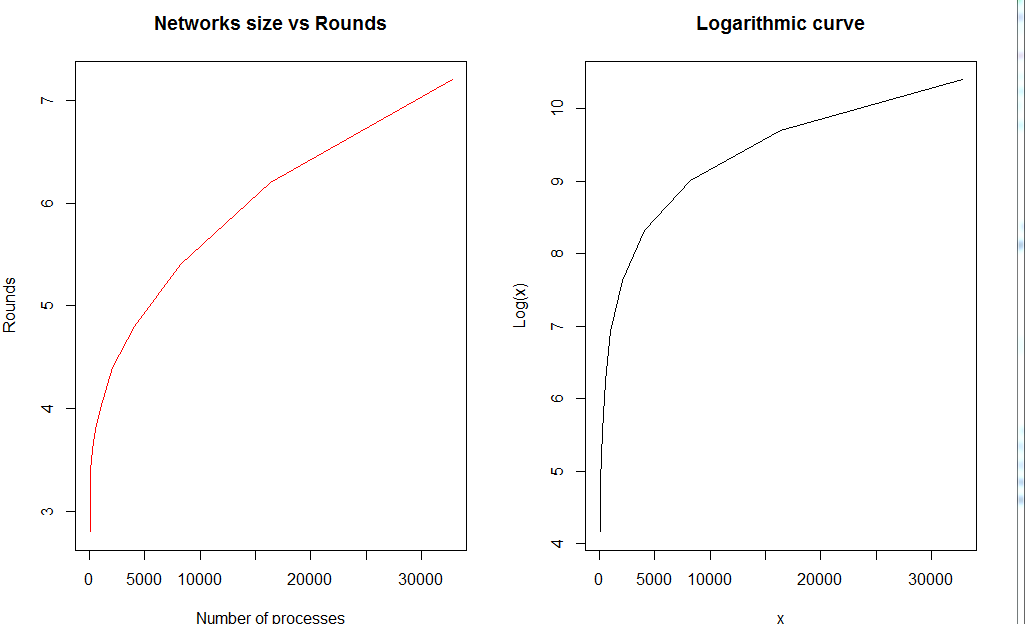
\includegraphics[width=1 \linewidth, height=5cm]{number_rounds.png} 
\caption{Rounds per execution}
\label{fig:rounds_execution}
\end{figure}

The progression of the algorithm can be seen in the figure \ref{fig:progression}. In each round a number of processes finish the execution and become inactive until all processes finish the execution and output the final state (\textit{MIS} member or not). The blue line the progression on the number of processes that output a \textit{MIS} member state per round and the red line show the number of processes that are neighbour of some process that is part of the MIS.  In the figure \ref{fig:actives}, the number of processes that are active in each round of a execution of 32768 processors. 

\begin{figure}[ht]
\centering
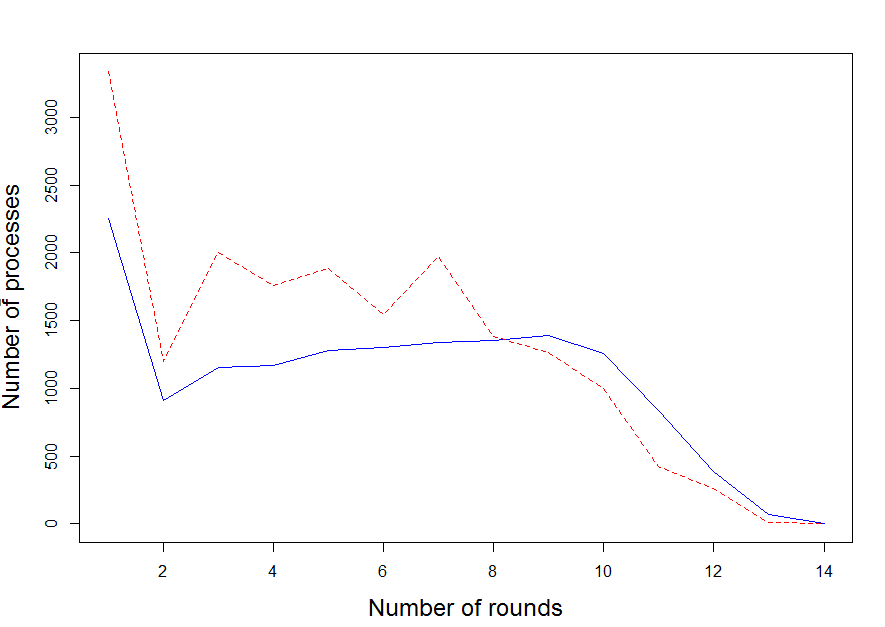
\includegraphics[width=0.7 \linewidth, height=5cm]{progress.PNG} 
\caption{Numbers of processes that finish the execution per round}
\label{fig:progression}
\end{figure}

\begin{figure}[ht]
\centering
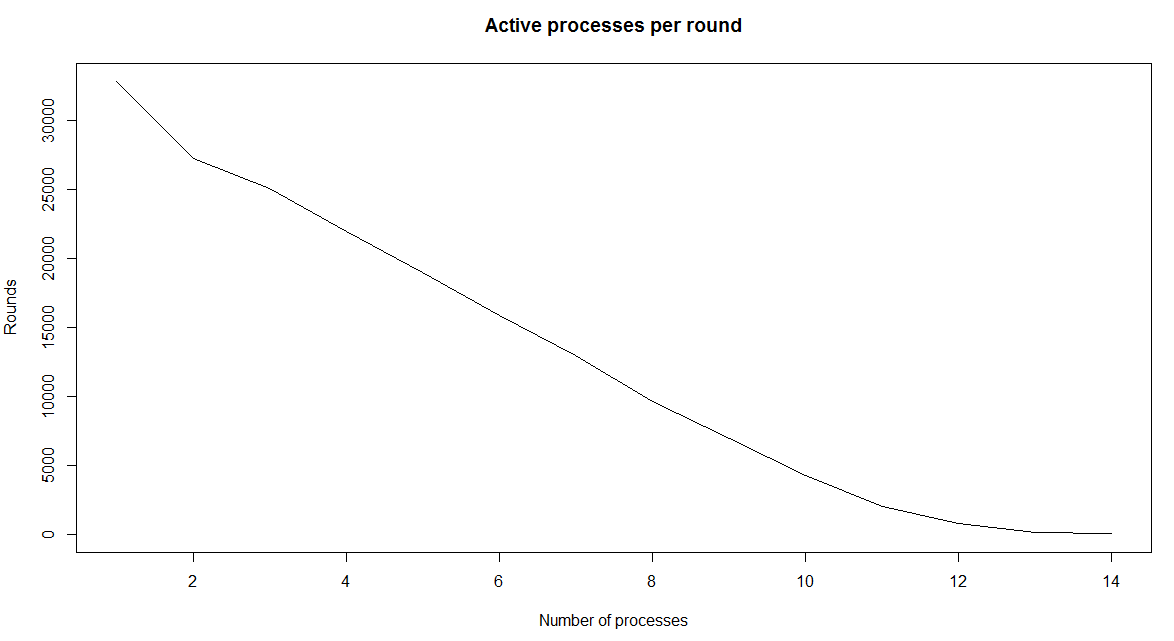
\includegraphics[width=0.7 \linewidth, height=5cm]{actives_round.PNG} 
\caption{Numbers of processes that finish the execution per round}
\label{fig:actives}
\end{figure}


\begin{figure}[ht]
\centering
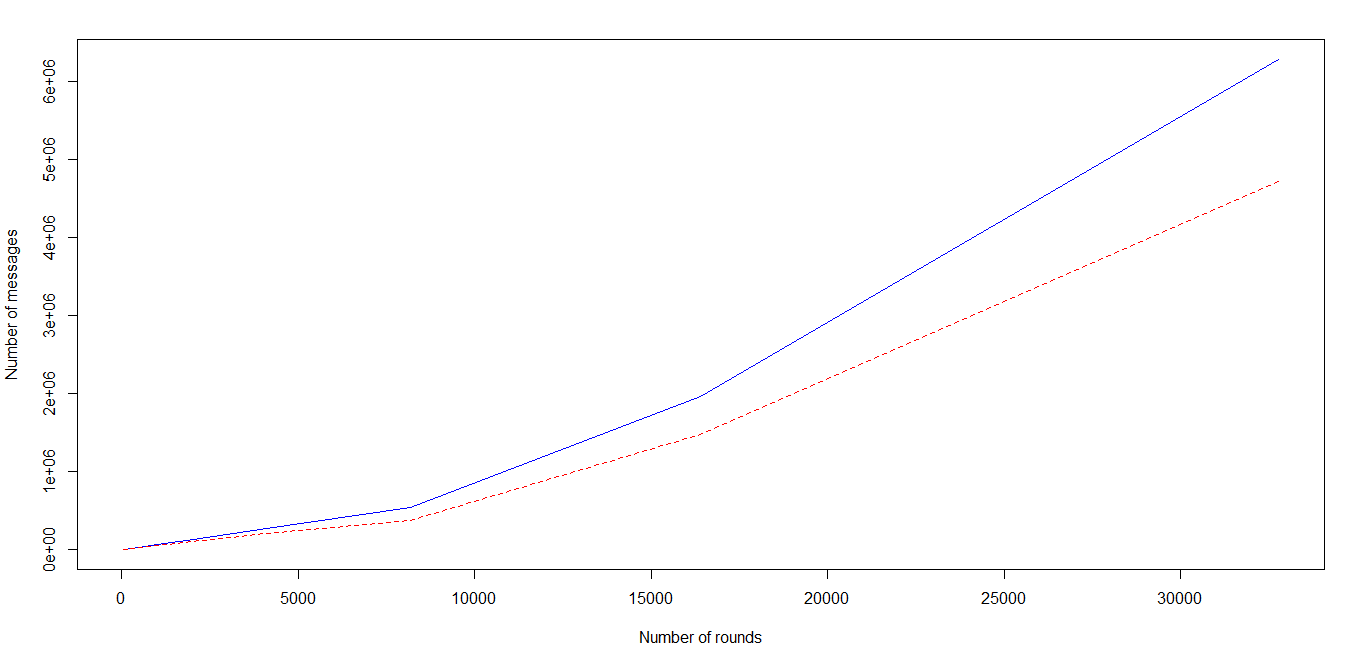
\includegraphics[width=0.7 \linewidth, height=5cm]{total_messages.PNG} 
\caption{Comparison between messages send for the protocol and the Global Synchronizer}
\label{fig:total_msg}
\end{figure}



\subsection{Evaluation of Synchronizers}